\chapter{Luminescent Organic Materials}
\label{chapter: luminscent organic materials}
%%%%%%%%%%%%%%%%%%%%%%%%%%%%%%
\section{Introduction}\label{section: lom introduction}
%%%%%%%%%%%%%%%%%%%%%%%%%%%%%%
Luminescent organic molecules are used in numerous biological and technological applications. In aqueous solution they are used extensively in biological imaging, probing, and detection. Deposited as thin films and aggregates, they represent the next generation of organic optoelectronics, where availability and low cost of starting materials, straightforward syntheses, and lightweight, flexible devices are attractive features. Perhaps most importantly, the luminescent response of molecular organic systems can be tuned with relative ease compared to their inorganic counterparts.

Since the discovery of electromluminescence in the 1960s, intensive efforts in academia and industry have delivered considerable progress in the field of organic electronics, leading to  the development of applications such as field-effect transistors, photovoltaic cells, optical memory devices, and single-crystal lasers.\cite{Ostroverkhova2016} The most prominent success story are certainly \acp{OLED}, which have already reached market adoption for lighting and display purposes. However, in many areas organic systems suffer from low efficiencies, trial-and-error optimisation, and decreased performance in aggregated form versus solution. 
To advance, there must be control over both the supermolecular structure of the material and the electronic structure of the  molecules within. Unfortunately neither of these properties exist in isolation, and the interplay between them must also be intimately understood, which somewhat complicates matters. Of these contributing factors, it is the electronic structure and its relationship with the environment which are of interest in this work. The luminescent response of molecules can change drastically from one medium to another, whether in the gas phase, as a solution, aggregated as clusters, or in molecular crystals. Understanding the interplay between the luminophore and its environment is crucial for designing more efficient materials from first principles. 

To this end, this work approaches the problem using theoretical chemistry methods to investigate organic compounds exhibiting \ac{AIE}. AIE-active compounds are non-emissive in dispersed media, but undergo a switch-on of luminescence, typically in the form of fluorescence, upon aggregation. Since technological applications require a thin-film or solid-state layer, AIE has attracted considerable interest as a pathway to overcome the common effect of \ac{ACQ}, hitherto a major obstacle in the development of organic luminophores. In this chapter the problem of \ac{ACQ} shall be introduced, followed by an examination of the AIE phenomenon through analysis of typical structures, mechanistic interpretations, before introducing the systems under investigation.
%%%%%%%%%%%%%%%%%%%%%%%%%%%%%%
\section{Aggregation Caused Quenching}\label{section: lom ACQ}
%%%%%%%%%%%%%%%%%%%%%%%%%%%%%%
Photoinduced luminescence occurs after chromophores with $\pi$-conjugation, typically in the form of aromatic moieties, absorb light in the UV/Vis region of the electromagnetic spectrum. In good solvents or dilute concentration, fluorescence will usually follow, although the presence of metals or second row elements can allow phosphorescence via intersystem crossing. Upon aggregation with increased concentration, or crystallisation, the fluorescence is often reduced or quenched completely. 

In 1954, photochemisty pioneer Theodor F\"{o}rster elegantly showed that the fluorescence of pyrene is shifted and weakened with increasing concentration (Figure \ref{figure: Forster_Spectra}).\cite{Forster1954,Forster1969} As the concentration increases, a new fluorescent species is formed and the original band loses intensity. The new band at longer wavelength is a result of the formation of excited dimers, or \textit{excimers}. The presence of aromatic rings in conventional luminophores leads to intermolecular $\pi$-$\pi$ interactions and the formation of dimers. In F\"{o}rster's pyrene example, where the spectra of differing concentrations are measured using the same incident wavelength, the single intersecting point shows that the spectrum consists of only two features. Since the absorption spectrum is unchanged in the concentration range, the arising band can be ``attributed to an associate that exists only in the excited electronic state, i.e. to an excimer."\cite{Forster1969}
\begin{figure}[H]
\centering
  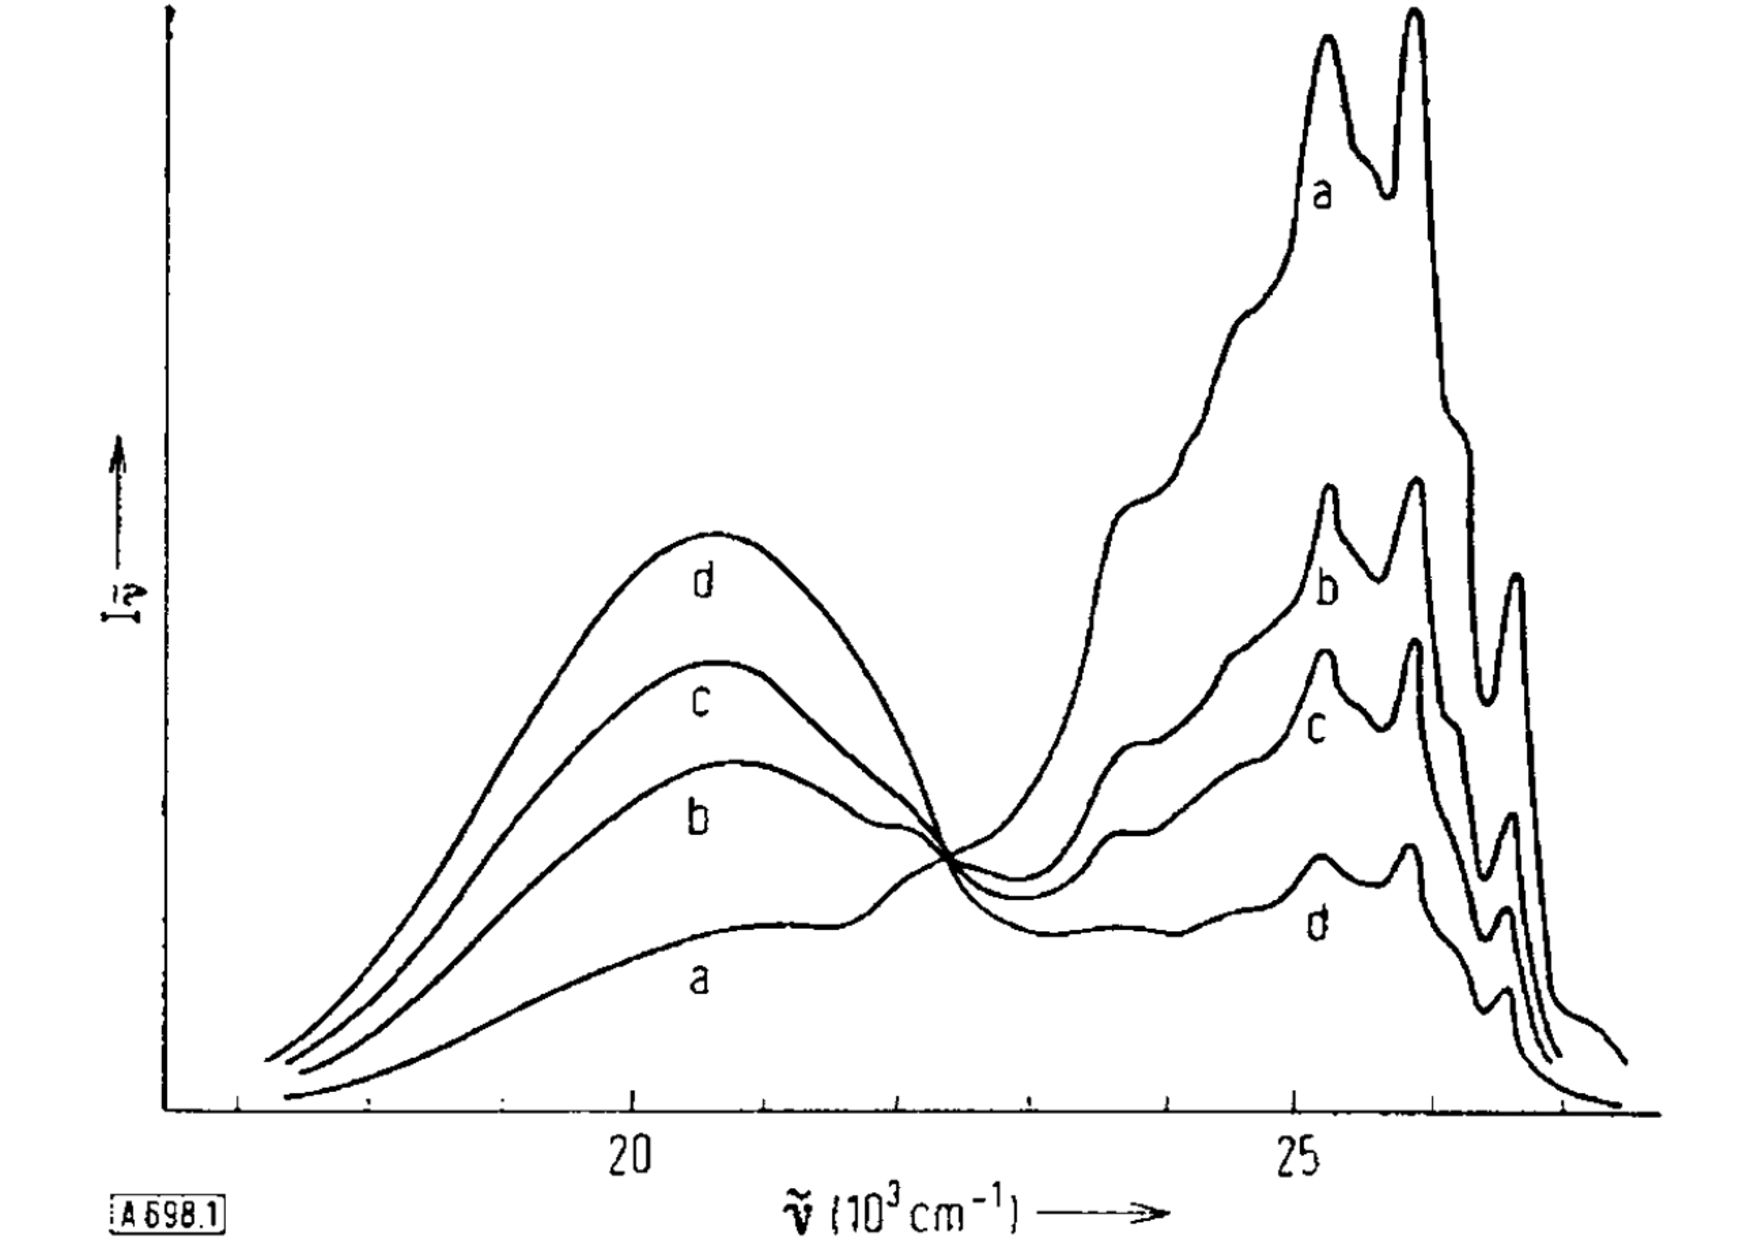
\includegraphics[width=0.6\linewidth]{Intro/Forster_Spectra.pdf}
  \caption[Fluorescence spectrum of pyrene]{Fluorescence spectrum of pyrene (in n-heptane, 20\degree{}C) at different concentrations: a) \SI{5.0e-5}, b) \SI{1.8e-4}, c) \SI{3.1e-4}, d) \SI{7.0e-4}{mol L^{-1}}. Reprinted from ref.~\citenum{Forster1969} with permission of Wiley-VCH.}
  \label{figure: Forster_Spectra}
\end{figure}
The supermolecular alignment of aromatic groups is commonly termed $\pi$-stacking or $\pi$-$\pi$ interactions in the chemical literature. However, this labelling can be slightly misleading and even inaccurate.\cite{Grimme2008,Martinez2012} Stefan Grimme argues that a specific $\pi$-$\pi$ interaction arises only in large, polyaromatic groups as a result of increased dispersion in specific orientations.\cite{Grimme2008} Meanwhile, a thorough review of experimental and theoretical literature by Martinez and Iverson found a lack of the face-centred stacking of aromatic groups which would maximise overlap of aromatic $\pi$ clouds.\cite{Martinez2012} They argue that the terms $\pi$-stacking and $\pi$-$\pi$ interactions are misnomers since they incorrectly imply the ubiquity of face-face stacking motifs. Typical stacking motifs are shown in Figure \ref{figure: Benzene_Stacking}, where parallel displacement tempers the unfavourable electrostatic interaction and reduces the Pauli exchange repulsion, with the dominating factor being the favourable dispersion interaction. Inclusion of substituents introduces a permanent dipole, with substituents preferentially aligning antiparallel.\cite{Martinez2012}

\begin{figure}[H]
\centering
  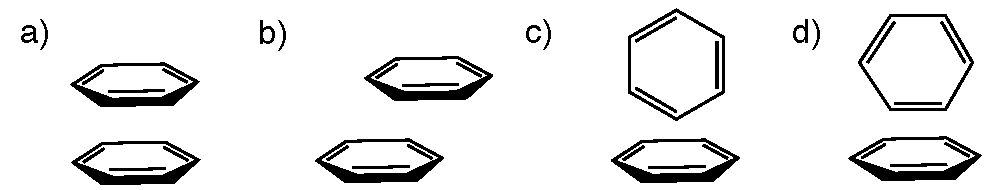
\includegraphics[width=0.7\linewidth]{Intro/Stacking.pdf}
  \caption[Stacking motifs of benzene]{Packing motifs of benzene molecules: a) face-centred, b) displaced, c) Perpendicular T-shaped, d) Perpendicular Y-shaped. Adapted from ref.~\citenum{Martinez2012}.}
  \label{figure: Benzene_Stacking}
\end{figure}

This intermolecular interaction is detrimental to solid-state fluorescence, and yet is a direct consequence of the design requirements of the chromophore. In biosensing applications, researchers resorted to using dilute solutions with reduced sensitivity because of \ac{ACQ}.\cite{Thomas2007,Kwok2015} In the solid state, for instance in thin films for optoelectronics, the \ac{ACQ} effect means that solution screening for viable candidates is rendered meaningless by the differing luminescent properties of the final material compared to the molecule. Strategies to circumvent \ac{ACQ} have seen varying success, for example through the inclusion of bulky substituents, polar groups, and promotion of hydrogen bonding.\cite{Hong2009,Zhang2013,Mei2014,Mei2015} However, synthetic modification can in turn effect the chromophore's electronic structure and its excited state properties, thus commencing tedious a trail-and-error optimisation process. Attempts to physically block aggregation by encapsulating in surfactants or polymer matrices require extensive engineering and can reduce charge transport.\cite{Hong2009,Chen2000,Lee2013} 

The deleterious effects of \ac{ACQ} cannot be underestimated and pose a significant problem for organic luminescent applications. In the next section of this chapter, we shall look in more detail of the photophysics of molecular aggregates, within the context of Kasha's exciton theory.
%%%%%%%%%%%%%%%%%%%%%%%%%%%%%%
\section{Photophysics of Molecular Aggregates}\label{section: lom intermolecular-interactions}
Intermolecular interactions become photophysically important in the solid state due to the dense packing of molecular units. This effect is typically framed in Kasha's two state exciton theory.\cite{Gierschner2009,Gierschner2013,Gierschner2013a,Hestand2017,Shi2017} The exciton is typically defined as a deloclised excited state, where the excited electron and hole remain in close proximity. The Coulomb interaction between the transition dipoles of the monomers in a dimer results in an energy shift in the absorption spectrum, and has underpinned exciton theory since its inception in the 1960s.\cite{Kasha1965a} When two monomers stack ``side-by-side", the Coulombic electronic coupling is positive, a blue-shifted absorption spectrum is witnessed (relative to the isolated monomer) and radiative decay is reduced. This stacking motif is denoted a H-aggregate. Conversely, in J-aggreagtes, dimers align ``head-to-tail", and a red-shifted absorption is witnessed with an increased radiative decay. These extreme cases have helped interpret the supermolecular photophenomena in molecular aggregates.

When the intermolecular distance is large enough to prevent orbital overlap, the exciton can be considered as the interaction of the wavefunction of one monomer ($\ket{1}$) with the wavefunction of the second monomer ($\ket{2}$). In the excited state, the  wavefunctions interact to form a delocalised exciton (a Frenkel exciton), the Hamiltonian $H$ of which is given
\begin{equation}
H=\hbar\omega + \mathrm{\hbar{}D} + J_{0}\{\ket{1}\bra{2}+\ket{2}\bra{1}\}.
\end{equation}
The first term is the energy gap between S\textsubscript{0} and S\textsubscript{1},  $\hbar{}D$ is the shift of the S\textsubscript{1} state in going from the vacuum to the crystal, and $J_{0}$ is the Coulombic coupling.\cite{Spano} The exciton for a multisite system can be described using periodic boundary conditions to produce a wavelike function $k$. For the two site system, $\ket{k}$ is\cite{Hestand2018}
\begin{equation}
\ket{k}=\frac{1}{\sqrt{2}}[e^{ik}\ket{1}+  e^{i2k}\ket{2}]\qquad\quad k=0,\pm{\pi}.
\end{equation}
For the allowed values of $k$, the transition energy $E_k$ for state $k$ is an eigenvalue of $H$, and has the form
\begin{equation}
\mathrm{E}_{k}=\hbar\omega + \mathrm{\hbar{}D} +J_{0}\cos{k}.
\end{equation}
For the two site system, this results in two exciton states in the Frenkel Hamiltonian, as depicted in Figure \ref{figure: H_J_Aggregates}. The Coulomb coupling $J_{0}$ represents the interaction energy due to exchange of excitation energy between $\ket{1}$ and $\ket{2}$, the sign of which dictates whether the symmetric superposition is the upper or lower state. When the coupling is positive, the symmetric state is the upper state, as in the H-aggregate, and the transition dipoles are reinforced resulting in absorption is blue-shifted compared to the gas-phase monomer. Since emission usually takes place from the lower state, where transition dipoles moments cancel, the state is nonradiative and fluorescence is quenched. When the coupling is negative, the symmetric state is lowered and emission is symmetry allowed.\cite{Hestand2017}
\begin{figure}[H]
\centering
  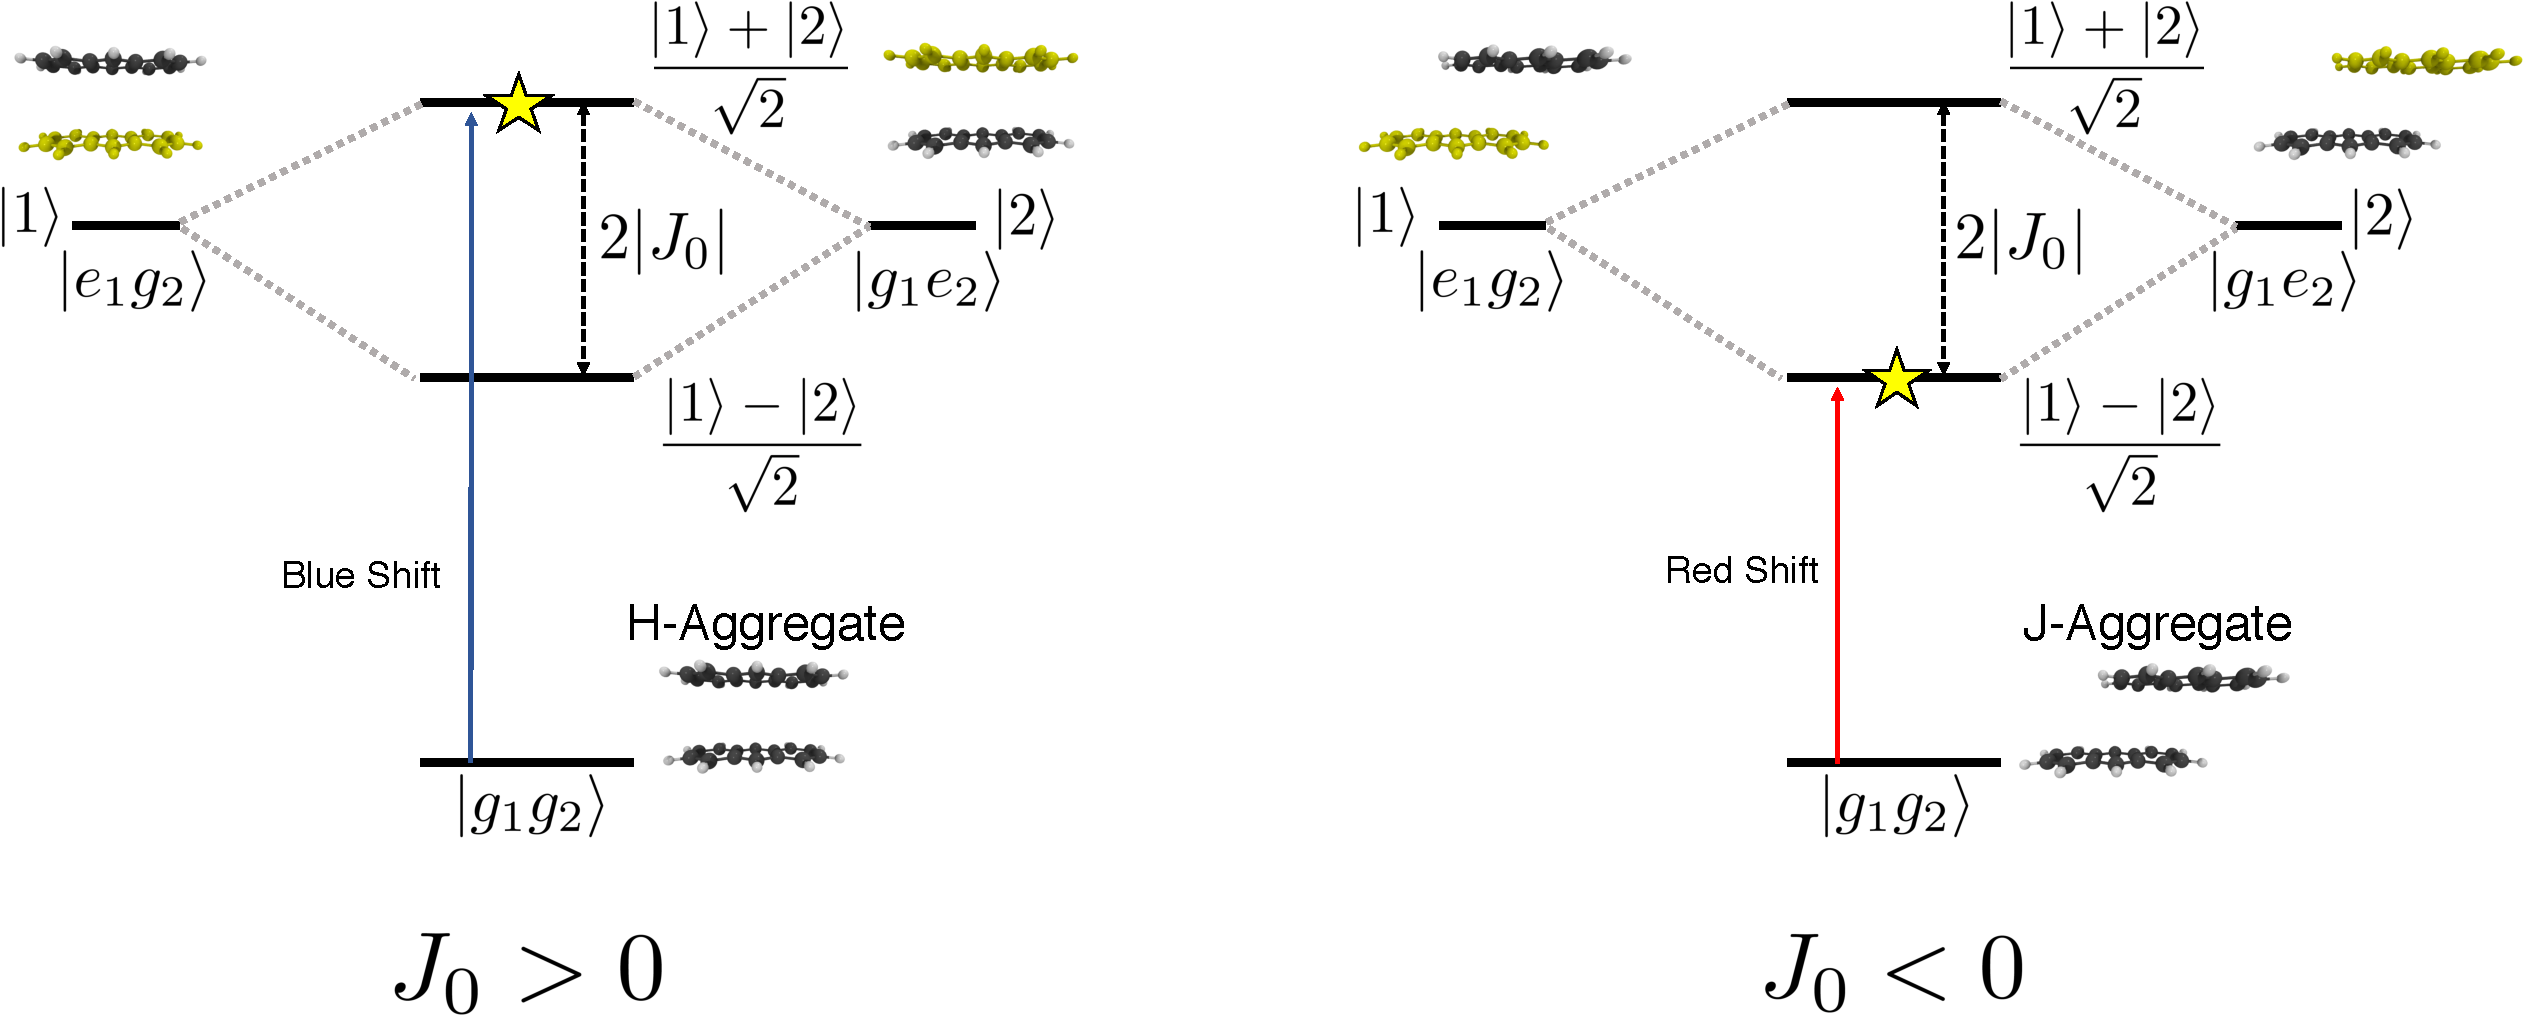
\includegraphics[width=\linewidth]{Intro/H_J_aggregates.pdf}
  \caption[Exciton energy level diagram for H- and J-aggregates]{Energy level diagram for a H-aggregate (left) and J-aggregate (right) of naphthalene. For the H-aggrgate, the Coulombic coupling $J_{0}$ is positive, raising the energy of the symmetric state resulting in blue-shifted absorption with respect to the monomer state. Emission from the lower state is forbidden, and thus quenched. In the J-aggregate, the negative Coulombic coupling results in red-shifted absorption and allowed emission. The bright excitonic state, the symmetric superposition of the monomer wavefunctions, is indicated with a star.}
  \label{figure: H_J_Aggregates}
\end{figure}
\begin{comment}
\begin{equation}
\ket{g_{1}g_{2}}
\end{equation}
\begin{equation}
\ket{e_{1}g_{2}}
\end{equation}
\begin{equation}
\ket{g_{1}e_{2}}
\end{equation}
\begin{equation}
J_{0}>0
\end{equation}
\begin{equation}
J_{0}<0
\end{equation}
\begin{equation}
2|J_{0}|
\end{equation}
\begin{equation}
\frac{\ket{1}+\ket{2}}{\sqrt{2}}
\end{equation}
\begin{equation}
\frac{\ket{1}-\ket{2}}{\sqrt{2}}
\end{equation}
\begin{equation}
\ket{1}
\end{equation}
\begin{equation}
\ket{2}
\end{equation}
\end{comment}
H- and J-aggregates represent the two extreme stacking cases. In Kasha's theory, the coupling $J_{0}$ arises from the interaction of the transition dipole moments, which at its most crude can be treated as the interaction between two point dipoles,
\begin{equation}
    J_{0,Coul}=\frac{\mu^{2}(1-3\cos^{2}\theta)}{4\pi\epsilon{}R^3}
\end{equation}
where $R$ is the intermolecular distance (between the centroids of the monomers), $\theta$ is the angle between  $\bm{\mu}$ (transition dipole vector) and $\bm{R}$, and $\epsilon$ is the optical dielectric constant of the medium. Thus for H-aggregates, when $\theta=90$, the coupling is positive, and is negative in J-aggregates when $\theta$ is close to zero. H-aggregates become J-aggregates at the so-called ``magic angle" of 54.7\textdegree.\cite{Hestand2018}

The crude point-dipole, Coulomb interpretation of the coupling is only valid approximation for homodimers with large intermolecular separation.\cite{Kistler2013} When monomers stack in close proximity ($R\leq4\si{\angstrom}$), wavefunction overlap invokes the possibility of \ac{CT} states, where the electron resides on one site and the hole on another.\cite{Darghouth2018} This creates a short-range coupling factor as well as the long-range Coulomb coupling. The total coupling is the combined short-range \ac{CT} coupling and the Coulomb coupling, leading to complex behaviour which is dependent on the sign of the short- and long-range contributions. For example, the \ac{CT} coupling is highly sensitive to the molecular geometry, where small distortions can change the total coupling value and result in multiple H- to J-aggregate conversions.\cite{Arago2015} The two components of the total coupling has lead to an expanded nomenclature for stacking motifs, where the contribution of both the short and long-range coupling is considered (HH, HJ, JH, JJ). In the JH and HJ, the interference is completely destructive and the total coupling is zero, resulting in an absorption spectrum at the same position as a monomer.\cite{Hestand2017}

Understanding the complex photophenomena of molecular aggregates is important in the development of materials requiring control over the exciton. The existence of exitons and the dynamics in the solid state, opens nonradiative decay channels and often a quenching of fluorescence for typical aromatic motifs. This has hindered the development of solid-state organic lumniscence. However, this changed when the group of Ben Zhong Tang found a system which had its fluorescence switched on, rather than quenched, upon aggregation - launching a new strategy for the design and development of brightly luminescent organic materials. They named the phenomenon  \acf{AIE}. In the next section of this chapter, the roots of \ac{AIE} shall be examined and the technological advances that have arisen from the discovery briefly outlined.

%%%%%%%%%%%%%%%%%%%%%%%%%%%%%%
%%%%%%%%%%%%%%%%%%%%%%%%%%%%%%
\section{Aggregation Induced Emission}\label{section: lom AIE}
%%%%%%%%%%%%%%%%%%%%%%%%%%%%%%
In 2001, the Tang group at the Hong Kong University of Science and Technology were interested in silole-based polymers for highly emissive thin-films. As was common at the time, fabrication of such materials was challenging due to \ac{ACQ}. Through serendipity during a purification process, they found that a wet spot of 1-methyl-1,2,3,4,5-pentaphenylsilole was almost non-emissive, but brightly fluorescent after solvent evaporation.\cite{Luo2001} The law of aggregation quenching emission had been turned on its head, and the Tang group had observed the exact opposite behaviour, of molecular aggregation inducing light emission. This was almost unheard of for small organic molecules. 

The Tang group used the \ac{AIE} phenomeon to develop a range of chemical sensors, to detect for instance volatile organic compounds, explosives, and pH.\cite{Dong2007,Li2005,Li2009} Such was the magnitude of the \ac{AIE} breakthrough and the mechanistic interpretations provided by the Tang group, many other groups began to explore this exciting new phenomenon for a wide range of applications. In the field of biological probing, \ac{AIE}-active systems can detect important small molecules such as glucose, thiols, and lactic acid.\cite{Wang2014,Yuan2014,Shen2012} Probes have been developed to detect protein fibrillation, which has been linked to Alzheimer's, Parkinson's and type II diabetes.\cite{Hong2012} \ac{AIE} systems have been also used in medical imaging, where fluorescence is an attractive technique due its high resolution, wide applicability, and low cost.\cite{Mei2015} The Tang group have tracked the progress of the field with periodic, in-depth reviews of the vast number of innovations, of which they contribute a significant share.\cite{Hong2009,Wang2010a,Hong2011,Mei2014,Hu2014,Mei2015}

Upon discovery of \ac{AIE}, the potential for the improvement of optoelectronic devices was immediately apparent. In the original publication, the group built a highly emissive blue-emitting electroluminescent device, and optimised the device to 8\% \ac{EQE} in the cyan region, a vast improvement on the previous high of just 1.5\% for an \ac{OLED}. \cite{Luo2001,Chen2002} \ac{EQE} is the product of the electroluminescence efficiency of the emitter (the organic layer in this case) and the external coupling factor, which is a measure of the fraction of light able to escape the \ac{OLED}. Due to electroluminescence efficiency being limited to 25\% for singlet emitters, and the external coupling being limited to around 22\%, it was previously thought that the theoretical maximum \ac{EQE} is 5.5\%. Indeed, such was the remarkable \ac{EQE} measure in this \ac{OLED} that these previously accepted limitations had to be reconsidered.

In follow-up work, a light-blue emitting \ac{OLED} with hexaphenylsilole (Figure \ref{figure: HPS_TPE}) as the emitting layer was fabricated with \ac{EQE} of 7\%.\cite{Chen2003} While the unfavourable spin statistics inhibit efficiency for singlet-emitting \acp{OLED} across the visible spectrum, deep blue emitters are harder still since the large band gap makes charge injection difficult, hindering the development of full colour displays. Non-doped deep blue \acp{OLED} with \ac{EQE} of around 4\% were reached in 2014, with emitters based on triphenylamine and tetraphenylethene (Figure \ref{figure: HPS_TPE}).\cite{Huang2014,Huang2014a} This has recently been increased to 6.5\% using a carbazole-based organic layer, and in 2018 reached 9.4\%.\cite{KumarKonidena2017,Tang2018} This represents a high for non-doped singlet blue emitters. Inclusion of phosphorescent or thermally-activated delayed fluorescent dopants can further increase the quantum efficiency by harvesting triplet states for luminescence.\cite{Zhu2018}

\begin{figure}[H]
\centering
  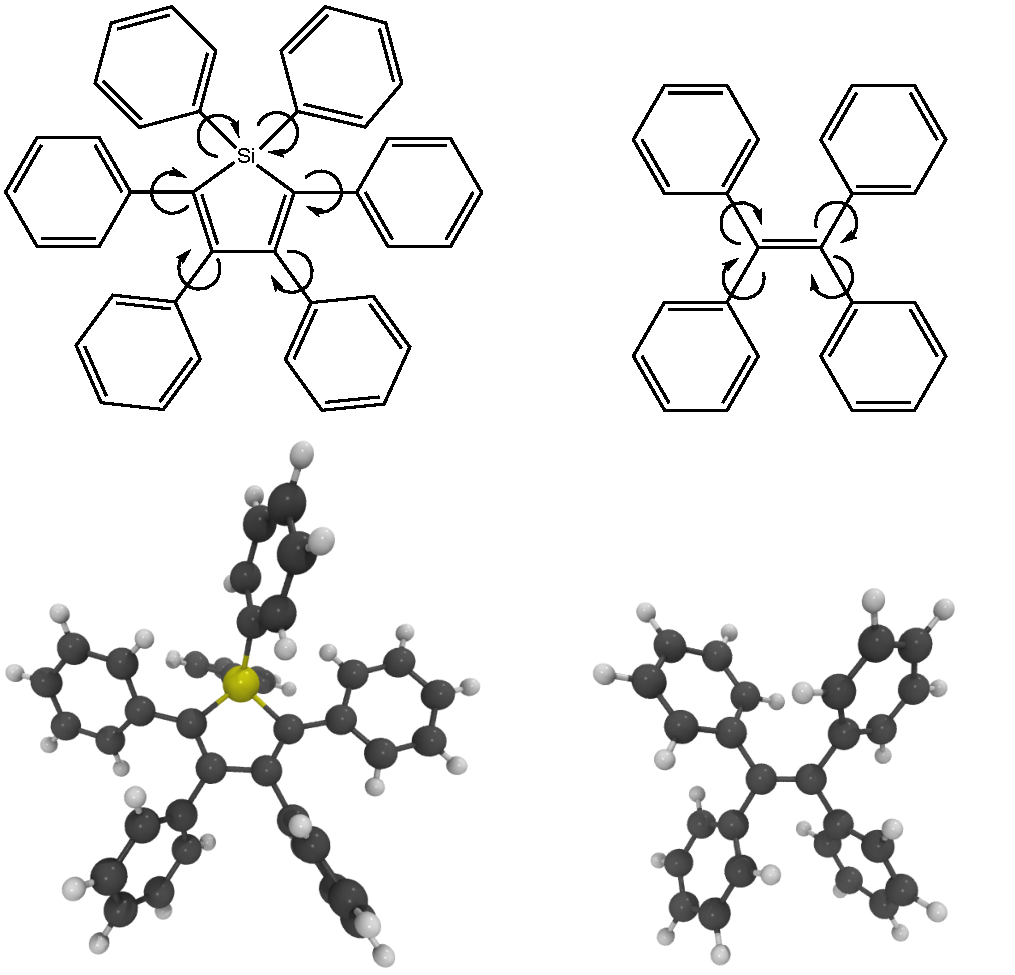
\includegraphics[width=0.7\linewidth]{Intro/HPS_TPE.pdf}
  \caption[Examples of AIE-active chromophores]{Two dimensional (top) and three dimensional (bottom) structures of two of the ubiquitous AIE-active systems, hexaphenylsilole (HPS, left) and tetraphenylethene (\ac{TPE}, right). AIE occurs through restriction of the rotational motions depicted with arrows.}
  \label{figure: HPS_TPE}
\end{figure}

Systems exhibiting \ac{AIE} are typically based on a propeller architecture, where a central stator is connected to a number of aromatic rotors via single bonds, as shown in Figure \ref{figure: HPS_TPE}. In the initial analysis of 1-methyl-1,2,3,4,5-pentaphenylsilole, the absorption spectra showed that after the water fraction in an ethanol-water solvent mixture rose above 60\%, the absorption band increased in intensity and moved to longer wavelengths.\cite{Luo2001} On this basis, the \ac{AIE} activity was attributed to the formation of aggregates which forced the molecules into a more planar conformation, thus increasing the conjugation and the absorption. Enough rotation about the sigma bonds was still possible to prevent complete planarity and therefore limiting the stacking and subsequent fluorescence quenching. 

A few months later, the group showed the \ac{AIE} effect for four more silole systems, followed by an extensive study of ten phenylsiloles.\cite{Tang2001,Chen2003} Crucially, in this later work the crystal structure of the siloles showed that the conformation remains twisted in the solid state.\cite{Chen2003} Large torsional angles exist between the phenyl groups and the central silole moiety, on account of the steric repulsion between the six phenyl groups. The lack of space between the phenyl blades, and their angular orientations, prevents intermolecular stacking which give rise to aggregation caused quenching. Therefore the planarisation hypothesis was wrong. 

The group investigated other quenching mechanisms, such as \ac{TICT}, where a non-emissive twisted conformer is formed via charge separation in the chromophore. The \ac{TICT} state can be stabilised, and thus favoured, in polar solvents. However, no emission was recorded across a wide range of solvent polarities for the siloles, ruling out \ac{TICT} as the cause for \ac{AIE}. Also, the lack of electron donor and acceptor groups make it highly unlikely that \ac{TICT} could take place in the siloles. In an elegant experiment it was found that the emission increased almost linearly with increasing solvent viscosity, even though no aggregates were formed. In a similar vain, the photoluminescence intensity increased with decreasing temperature, with NMR studies confirming that the intramolecular rotations of the exterior phenyl groups were reduced at lower temperatures. It was concluded the in good solvents, at ambient temperature, the energy consumed by the rotation of the phenyl groups about the single bonds results in the nonradiative decay of the excited state decay. Upon aggregation, the propeller-like shape limits the intermolecular stacking. Strong C-H\textperiodcentered\textperiodcentered\textperiodcentered$\pi$ interactions rigidify the structure, hindering the intramolecular rotation and the excited state decays via fluorescence.\cite{Chen2003}

The \ac{RIR} mechanism allowed the library of \ac{AIE}-active systems to be expanded to other molecules with propeller-shaped structures. Along with the phenylsiloles, \ac{TPE} derivatives (Figure \ref{figure: HPS_TPE}) have driven understanding and technological progress in the field.\cite{Hong2009,Wang2010a,Hong2011,Mei2014,Hu2014,Mei2015} By switching a phenyl group of \ac{TPE} with a traditional \ac{ACQ} molecules, such as triphenylamine or carbazole, the electroluminscence properties of the system are enhanced due to the hole-transport properties of the \ac{ACQ} group.\cite{Chan2014} Conversely, \ac{ACQ} cores can be made to undergo \ac{AIE} by the attachment of \ac{TPE}.\cite{Yuan2010a}

Dissipation of the excited state can occur through means other than rotation. A bent, $\pi$-surface system of benzenes fused with cyclooctatetraenes undergoes \ac{AIE} but without any rotable units.\cite{Nishiuchi2013} In solution, ring inversions dissipate the excited state and there is almost no emission. Single crystals show emission in the blue region, since the bent structure prevents facial stacking and the inversion modes are restricted. Thus \ac{AIE} is achieved through \ac{RIV}. In a similar vain, the \ac{RIV} mechanism can be applied to \ac{TPE} by locking pairs of phenyl groups with eythlene linkers. In 2014, Tang unified the \ac{RIR} and \ac{RIV} interpretations under the \ac{RIM} umbrella.\cite{Leung2014}

The discovery and development of the \ac{AIE} phenomenon has transformed the field of luminescent organic materials. While much of the innovation has been based on the propeller systems, a class of systems based on \ac{ESIPT} have attracted interest in recent years for their favourable photochemical properties. \ac{ESIPT} systems form the basis of the research in this thesis and in the next section the \ac{ESIPT} mechanism shall be introduced, along with the key applications which incorporate \ac{ESIPT}.
%%%%%%%%%%%%%%%%%%%%%%%%%%%%%%
\section{Excited State Intramolecular Proton Transfer}\label{section: lom ESIPT}
%%%%%%%%%%%%%%%%%%%%%%%%%%%%%%
Tautomerism is a type of isomerism resulting in the transfer of a chemical group (usually a proton) between two sites on a molecule, and the simultaneous switching of a single and double bond. Photo-induced tautomerism, where the transferring group is a proton, is called \acf{ESIPT}. Research into the mechanism and potential applications of ESISPT has been active for more than half a century, since \ac{ESIPT} was first observed in the 1950s in salicylic acid. Photochromic materials harnessing \ac{ESIPT} have garnered much attention due to the wide range of applications and remarkable properties. In particular, it is the unusually large Stokes-shifted emission which makes \ac{ESIPT} so attractive. The separation between the absorption and emission wavelengths can typically exceed 200 nm, reducing self-absorption and increasing the output signal for the desired application. The emission colour can be tuned by the addition of electron donating or withdrawing groups, as well as solvent polarity and viscosity.\cite{Azarias2016,Yushchenko2007} Dual emission from the pre- and post-\ac{ESIPT} forms is also possible. These characteristics, in tandem with \ac{AIE}, have resulted in \ac{ESIPT} chromophores being used for chemical sensing, biological imaging and probing, as well the optoelectronic applications such as optical memory, lasers, and \acp{OLED}.\cite{Hsieh2010,Kwon2011,Zhao2012,Demchenko2013,Padalkar2015,Chen2018}
\begin{figure}[H]
\centering
  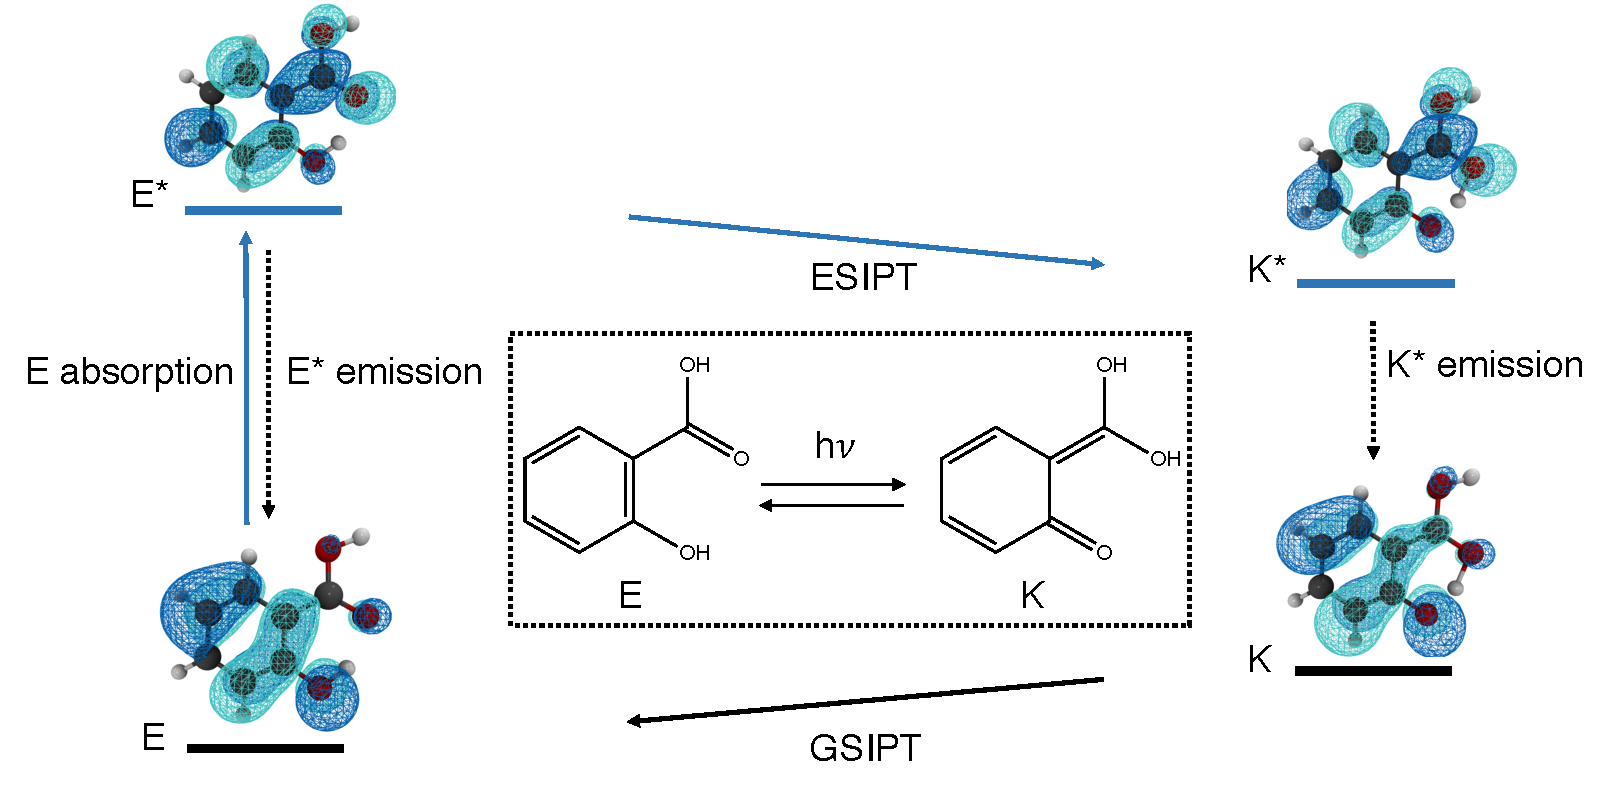
\includegraphics[width=0.95\linewidth]{Intro/ESIPT.pdf}
  \caption[The four-level photocycle of \ac{ESIPT}]{The four-level photocycle of \ac{ESIPT} for salyclic acid. The HOMO and LUMO orbitals for tautomer are also shown.}
  \label{figure: ESIPT}
\end{figure}
Inherent in all \ac{ESIPT} processes is a fully reversible four-level photocycle, the prerequisite for which is the presence of an intramolecular hydrogen bond. The proton donor can be an amino or hydroxyl group, while the proton acceptor is usually an imine or carbonyl. The four-level photocycle for salicylic acid is depicted in Figure \ref{figure: ESIPT}, along with the main molecular orbitals. The chromophore in the ground state (S\textsubscript{0}) is in the enol form (E), mediating hydrogen bond formation between the carbonyl oxygen and the hydroxyl proton. Upon electronic excitation, the excited state (E$^\ast$, S\textsubscript{1}) the geometry remains unchanged but electronic redistribution acidifies the hydroxyl and increases the basicity of the carbonyl group, as a result of the population of the $\pi^\ast$ orbital on the carbonyl oxygen. In the excited state, the keto form (K$^\ast$) is more stable due to the redistributed electron density, and the proton migrates from the hydroxyl oxygen to the carbonyl oxygen. Depending on the system, fluorescence can occur from both the excited enol form (E$^\ast$) and the excited keto form (K$^\ast$), although due to the ultrafast nature of the proton transfer the major emitting species is the keto tautomer.\cite{Zhao2012} For most \ac{ESIPT} processes containing strong hydrogen bonds, proton transfer is near barrierless and  occurs on a femtosecond time scale.\cite{Padalkar2015} The rate of the proton transfer and emission wavelength are highly sensitive to the surrounding medium and the presence of electron donor/acceptor moieties.\cite{Demchenko2013,Lin2017a,Li2017c} After fluorescence, the ground state keto form (K) is populated and the four level photocycle (E$\rightarrow$E$^{\ast}$$\rightarrow$K$^{\ast}$$\rightarrow$K) is completed. The initial geometry is restored through \ac{GSIPT}, although other photoproducts can be formed, for instance through cis-trans isomerisation or intersystem crossing.\cite{Al-Soufi1990}

\ac{AIE} in \ac{ESIPT} chromophores can be more complex than in non-polar propeller systems. The presence of hydrogen bonding sites enables the formation of intermolecular hydrogen bonds with solvent molecules, weakening the intramolecular bond and hindering \ac{ESIPT}.\cite{Cheng2015f} Kasha showed that the ratio of fluorescence intensity between E$^\ast$ and K$^\ast$ dramatically changes based upon the solvent polarity.\cite{Kasha1986} In 3-hydroxyflavanone, the K$^\ast$ fluorescence band is suppressed and the E$^\ast$ band increases in intensity with polar solvents. In strongly basic solvents, intermolecular proton transfer can occur between the chromophore and solvent, blocking access to the K$^\ast$ state\cite{Laurent2014}. As touched upon earlier, the presence of donor acceptor groups opens the possibility of deactivation through \acf{TICT}. In solvent, the \ac{TICT} state is populated after proton transfer and lead to nonradiative decay. In a similar vain to \ac{RIR}, aggregation frustrates the torsional mode, preventing the \ac{TICT} from forming, and opens the radiative decay channel.\cite{Park2017,Wu2015a}

The most investigated class of \ac{ESIPT} molecules are based on benzothiazole dyes, particularly \ac{HBT}.\cite{Padalkar2015,Kwon2011} The groups of Li and Liu investigated the effect of solvent for a range of \ac{HBT} derivatives, finding that increasing polarity impedes the proton transfer reaction and diminishes fluorescence. This is compounded by highly polar, protic solvents, where the hydroxyl proton can dissociate to form the phenolic anion. The proton transfer is highly sensitive to the solvent polarity, which is highly useful for sensing and probing applications.\cite{Wang2009,Cheng2015f} A \ac{HBT} analogue has been developed for ratiometric probing for hydrogen peroxide in living cells, where the \ac{ESIPT}-active fluorophore is produced by oxidative hydrolysis.\cite{Tang2018a} \ac{HBT}-based systems are also applicable for pH sensing, ion detection, biothol probing, and intracellular imaging.\cite{Kachwal2018,Kachwal2018,Liu2018}

Substitution of electron donor and acceptor groups onto \ac{ESIPT} cores can alter the proton transfer rate and stability of the enol and keto conformers on the excited state potential energy surface. In an extensive theoretical study, Jacquemin and co-workers investigated how different substitution patterns affect the emission from enol and keto states for a range of benzothiazoles.\cite{Azarias2016} They found that dual emission from both E$^*$ and K$^*$ is only possible in a small energy window for the compounds tested, and that the K$^*$ minimum can be favoured more drastically by dependent on the heteroatom in the core. The strongest substituent effects are seen with electron donor groups, such as methoxy, which stabilise the E$^*$ state. The K$^*$ state can be favoured by electron withdrawing groups in particular positions. Crucially, the effects of combining substituent groups is complex and depend on the specific \ac{ESIPT} core and substituent combination. The easily purturbed electronic structure of these systems make design from first principles extremely challenging.

\ac{ESIPT} cores are excellent candidates for optoelectronic applications on account of minimised self-absorption. However, the environment sensitivity which makes them so suitable for probing can be harmful to device stability.\cite{Kwon2011} Through chemical modifications, the Park group have fabricated stable \ac{OLED} devices with a range of emission frequencies.\cite{Park2008,Park2009,Kim2011} Introduction of carbazole gave access to blue K$^*$ emission, while \ac{EQE} values of 14\% have been reached by incorporating triplet harvesting via thermally activated delayed fluorescence with \ac{ESIPT}.\cite{Park2008,Mamada2017} Emission from both E$^*$ and K$^*$ enables white-light emission in devices, a highly attractive property due to the rarity of single molecule fluorophores with wide emission bands.\cite{Tang2011,Yao2011,Zhang2016b,Serdiuk2017}

The population inversion afforded by the K$^\ast$ form makes \ac{ESIPT} systems attractive for laser applications.\cite{Fang2014,Gierschner2016} Additionally the large Stokes shift limits reabsorption and increases the optical gain.\cite{Kwon2011} In the 1980s, the principle of using \ac{ESIPT} for lasing applications was established by Kasha and co-workers for 3-hydroxyflavone, where the ultrafast proton transfer and double-well excited state potential energy surface lead to efficient population inversion.\cite{Khan1983,Chou1984} Since then, the structural diversity of \ac{ESIPT} systems have produced lasers with emission in the green, orange, and cyan regions.\cite{Sakai2016,Chen2016,Park2012,Park2008} Recently, an imidazole-based system with amplified spontaneous emission properties was developed with deep blue emission.\cite{Park2017} The restriction of the \ac{TICT} state in the crystalline form results in quantum yield of fluorescence of 67\%, producing an intense and narrow blue band for emission. 

Developing efficient fluorophore emission at the extremes of the visible spectrum is notoriously difficult. Whilst much attention has been paid to the blue region, the red and \ac{NIR} region is also hugely challenging in the solid state. The first system to exhibit solid state lasing properties in the \ac{NIR} region was reported in 2015.\cite{Cheng2015} The compounds were based on \ac{HC} skeletons and displayed \ac{ESIPT}. Interestingly, solid state fluorescence is only witnessed in some analogues, with substituent position and crystal packing modes determining the quantum yield of fluorescence. The question of whether electronic effects or the crystal structure determined the fluorescence activity was not fully resolved. Fluorene-containing derivatives with laser properties were published soon after.\cite{Cheng2016} In the same year, the same group published another breakthrough in solid state lasing, with structures based on  \ac{HP}.\cite{Tang2016} These compounds are similar to the \acp{HC}, but contain only one aromatic ring. Solid state fluorescence in single-benzene emitters is a rarity due to low melting points, but these systems showed extremely high fluorescence activity, surpassing the parent \ac{HC} systems.

For the \ac{HC} and \ac{HP} systems, the crystal packing, absorption and emission wavelength, andcrucially the QE, are all dependent on the choice of substituent and number of aromatic rings. How these factors interplay is not well understood. To fully understand the photophysical properties of these systems, intricate knowledge of the electronic, molecular picture must be combined with the intermolecular interactions inherent in the crystal as a whole. Theoretical methods can help elucidate this picture and offer insight into the working mechanisms behind \ac{AIE} for these \ac{ESIPT} systems, and how to maximise the quantum yield of fluorescence. This is the primary aim of the work in this thesis, with \ac{HC} and \ac{HP} families used as exemplars. In the next section, the properties of \ac{HC} and \ac{HP} shall be examined, with main focus on the parent \ac{HC} compounds. 
%%%%%%%%%%%%%%%%%%%%%%%%%%%%%%
\section{Emitters based on 2'-hydroxychalcones}\label{section: lom HC}
%%%%%%%%%%%%%%%%%%%%%%%%%%%%%%
Research into \acp{HC}, and chalcones in general, has traditionally revolved around their metabolite character, since they are in vivo precursors for a variety of flavones, flavonols, isoflavones, anthocyanidins, and other synthetic antioxidants.\cite{Singh2014} \acp{HC} also show \ac{ESIPT} fluorescence in the \ac{NIR} region upon aggregation. The \ac{ESIPT} process in \ac{HC} was first proven by Chou et al. in 1992.\cite{Chou1992} With an absorption band at 354 nm, and emission at 635 nm, the authors concluded that tautomerisation occurs upon absorption and that the keto S\textsubscript{1} state was responsible for emission. Cis-trans isomerism about the central double bond followed by molecular oxygen incorporation produces the flavanoid studied by Kasha, 3-hydroxyflavone. Previous studies had investigated this cyclisation mechanism, where it was initially thought cyclisation occurred through cis-trans isomerisation without proton transfer.\cite{Stermitz1975,Matsushima1985} It was later found that this isomerism could be hindered by solvent viscosity.\cite{Tokumura1998} Later, Arai and coworkers investigated the photochemistry of \textbf{HC} analogues, where they denoted the tautomerisation to be hydrogen atom transfer, rather than proton transfer.\cite{Arai1997,Norikane2002,Norikane2003,Kaneda2003,Kaneda2003a,Kaneda2004,Teshima2009} They mapped the potential energy surfaces using spectroscopic techniques to find that the cis-trans isomerism takes place in the triplet state, and only after hydrogen atom transfer. Most pertinent was their study of the effect of substituent on fluorescence in 2009.\cite{Teshima2009}  Studying systems solvated in benzene, they found that the addition of a methoxy substituent in the para position of the phenol ring increased the quantum yield of red fluorescence by at least ten times, which the authors attribute to a combination of electronic and steric effects. The methoxy group stabilises the S\textsubscript{1} state through electron donation to the carbonyl $\pi\pi^\ast$ orbital whilst its size hinders the intramolecular modes. 

More recently, \textbf{HC} compounds have been developed for sensing and imaging applications. In 2014, the Tang group (of \ac{AIE} fame), developed a ratiometric fluorescent probe for sensing alkaline phosphatase based on 2'-hydroxychalcone.\cite{Song2014} Alkaline phosphotase is a dephosphorylating  enzyme, high concentration of which acts as a biomarker for diseases such as hepatitis, prostate cancer, and bone issues. By replacing the hydroxyl group of \textbf{HC} with a phosphoric acid group, the emission is yellow in aqueous conditions. In the presence of alkalane phosphotase, the cleave of phosphate and yields 2'-hydroxychalcone, which undergoes \ac{ESIPT} and emits in the red region. Another probe was developed to detect cysteine, again through the activation of \ac{ESIPT}.\cite{Li2017a} The \ac{AIE}/\ac{ESIPT} principle was applied using \textbf{HC} to develop a technique to detect latent fingerprints, for example in crime scenes.\cite{Jin2015} A fingerprint contains a high level of sebum, and when this is rinsed a \textbf{HC} solution, the \textbf{HC} molecules preferentially adhere to the fatty acid residues in the fingerprint, where they aggregate. When light is shone on the fingerprint, \ac{ESIPT} occurs and red fluoresence is produced, lighting up the fingerprint region against the dark backdrop of the substrate. 

In 2015, Zhang et al. synthesised a range of crystalline \textbf{HC} systems with different substitution patterns.\cite{Cheng2015} They found the identity and the position of the substituent to be critical in the quantum yield of the crystals. This is summarised in Figure \ref{figure: HC_experimental}. When substituents are meta to  the hydroxyl group (compounds \textbf{1}-\textbf{3}) in the phenol ring, deep red fluorescence is observed, but only when in crystalline form. The solutions are almost non-emissive. Interestingly, under frozen conditions the solutions still only weakly fluoresce, indicating that restriction of intramolecular rotation is not the key factor in the \ac{AIE} for these molecules. When the same substituents are in para position (compounds \textbf{4},\textbf{5}), neither the crystals nor the solutions are emissive. 
\begin{figure}[H]
\centering
  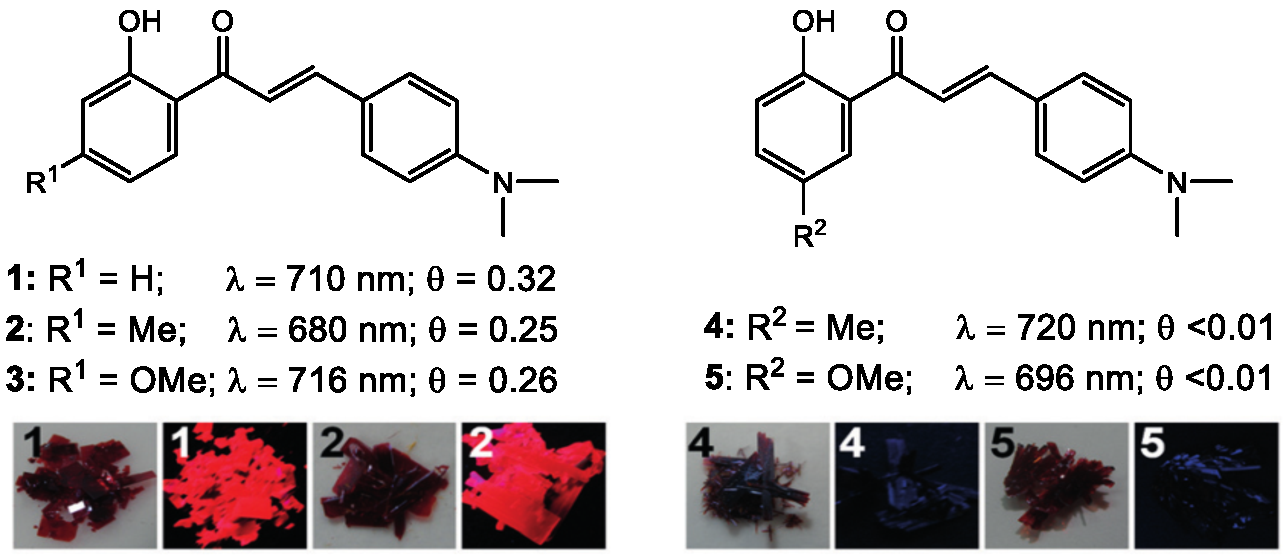
\includegraphics[width=0.95\linewidth]{Intro/HC_experimental.pdf}
  \caption[Emission behaviour of crystalline 2'-hydroxychalcone derivatives]{Compounds \textbf{1}-\textbf{5} synethised by Zhang and coworkers. \textbf{1}-\textbf{} show high quantum yield, but \textbf{4}\&\textbf{5} are almost non-emissive. Absorbance maxima ($\lambda$) and quantum yields of fluorescence ($\theta$) are given, along with pictures of the dark and bright crystals for \textbf{1},\textbf{2},\textbf{4}, and \textbf{5}. Figure adapted from ref.~\citenum{Cheng2015} with permission of Wiley-VCH.}
  \label{figure: HC_experimental}
\end{figure}
These puzzling characteristics are attributed to both the planarity of the individual molecules and the packing in the crystal, as shown in Figure \ref{figure: HC_stacking}   Molecules \textbf{1}-\textbf{3} are almost completely planar and the strong intramolecular H-bonds, of length 1.753-1.780 \si{\angstrom}, increase the rigidity and planarity of the system. In the crystal, the molecules adopt an edge-to-face, herringbone packing mode preventing intermolecular $\pi$-interactions between the aromatic rings and enabling fluorescence from the keto S\textsubscript{1} state. For compound \textbf{4}, where a methyl substituent is para to the hydroxyl, a similar edge-to-face packing mode is present. However, the molecule has a larger dihedral angle than \textbf{1}-\textbf{3}, which the authors attribute as the reason for the weak fluorescence. For \textbf{5}, the molecule is planar but the packing is face-to-face with aromatic stacking interactions. In the discussion, it is asserted that \textbf{5} is therefore non-emissive in the solid state due to excimer formation and non-radiative decay. The authors also hypothesise that the edge-face packed crystal of compound \textbf{4} shows minimal fluorescence because the molecule is not planar, despite other edge-face packed molecules brightly fluorescing, while the planar molecule does not emit because it is packed face to face.
\begin{figure}[H]
\centering
  \includegraphics[width=0.95\linewidth]{Intro/HC_stacking}
  \caption[Crystal structures of 2'-hydroxychalcone derivatives]{The conformation of monomers \textbf{1},\textbf{4}, and \textbf{5}, along with their crystal structure. Crystal structures obtained from CCDC database codes from ref.~\citenum{Cheng2015}.}
  \label{figure: HC_stacking}
\end{figure}
It is with these hypotheses that this thesis begins. The first fundamental question is why do none of the five compounds fluoresce in good solvent? Secondly, in the solid state, why do only compounds \textbf{1}-\textbf{3} exhibit \ac{AIE}. Is this a substituent effect, as a result of the position of the methyl and methoxy groups, or is it due to the molecular packing mode, or is it a combination of both? Quantum chemical methods can identify the nonradiative decay channels in both dispersed and aggregated states, and therefore can elucidate the discrete electronic and intermolecular factors. In answering these questions, we can build understanding of how structure-property relationships operate in the \ac{AIE}/\ac{ESIPT} space. 
%%%%%%%%%%%%%%%%%%%%%%%%%%%%%%
\section{Structure of thesis}\label{section: lom outline}
%%%%%%%%%%%%%%%%%%%%%%%%%%%%%%



